\chapter{Port-Hamiltonian plate theory}

\epigraph{You get tragedy where the tree, instead of bending, breaks.}{\textit{Culture and Value\\
Ludwig Wittgenstein}}
\minitoc

\lettrine{\color{theme}{P}}lates are plane structural elements with a small thickness compared to the planar dimension. Thanks to this feature, it is not necessary to model plate structures using three-dimensional elasticity. Dimensional reduction strategies are employed to describe plate structures as two-dimensional problems. These strategies rely on an educated guess of the displacement field. For beams and plates this field is expressed in terms of unknown functions $\phi_i^j(x,y,t)$ that solely depends on the midplane coordinates $(x,y)$
\begin{equation*}
u_i(x,y,z,t) = \sum_{j=0}^m (z)^j \phi_i^j(x,y,t).
\end{equation*}
where $u_{i}, \, i = \{x, y, z\}$ are the components of the displacement field. A first-order approximation is commonly used, meaning that a linear dependence on $z$ is considered. Two main models arise from such a framework: 
\begin{itemize}
	\item the Mindlin-Reissner model for thick plates;
	\item the Kirchhoff-Love model for thin plates.
\end{itemize}

In this chapter it its shown how to formulate first-order plate models as pHs. 

\section{First order plate theory}
As previously stated, first order theories assume a linear dependence on the vertical coordinate (cf. \cite{reddy2006theory})
\begin{equation*}
u_i(x,y,z,t) = \phi_i^0(x,y,t) + z \phi_i^1(x,y,t).
\end{equation*}
This hypothesis implies that the fibers, i.e. segments perpendicular to the mid-plane before deformation, remain straight after deformation. Additionally, for plate with moderate thickness the fibers are considered inextensible, meaning that $\phi_z^1 = 0$. These assumptions lead to the following displacement field

\begin{equation}\label{eq:disp1or}
\begin{aligned}
u_x(x,y,z,t) &= u_x^0(x,y,t) -z \theta_x(x,y,t), \\
u_y(x,y,z,t) &= u_y^0(x,y,t) -z \theta_y(x,y,t), \\
u_z(x,y,z,t) &= u_z^0(x,y,t), 
\end{aligned}
\end{equation}
where $u_i(x,y,t) = \phi_i^0(x,y,t), \, \theta_i(x,y,t) = -\phi_i^1(x,y,t)$. Assuming a linear elastic behavior, the 3D strain tensor for such a displacement field takes the form
\begin{align}
\varepsilon_{\alpha \beta} &= \frac{1}{2} \left(\partial_\beta u_\alpha + \partial_\alpha u_\beta \right) - z \frac{1}{2} \left(\partial_\beta \theta_\alpha + \partial_\alpha \theta_\beta \right) = {\varepsilon}^0_{\alpha \beta} - z \kappa_{\alpha \beta}, \label{eq:eps_inplane}\\
\varepsilon_{\alpha z} &= \frac{1}{2} \left(\partial_a u_z - \theta_\alpha \right) = \frac{1}{2} \gamma_\alpha,
\end{align}
where $\alpha=\{x,y\}, \; \beta=\{x,y\}$. The tensors $\bm{\varepsilon}^0,\, \bm{\kappa},\, \bm{\gamma}$ are called membrane, bending (or curvature) and shear strain tensor
\begin{align}
\bm{\varepsilon}^0 &= \Grad \bm{u}^0, \label{eq:eps0} \\
\bm{\kappa} &= \Grad \bm{\theta}, \label{eq:kappa}  \\
\bm{\gamma} &= \grad u_z - \bm{\theta}. \label{eq:gamma}
\end{align}
where $\bm{u}^0 = (u_x, u_y)^\top, \; \bm{\theta} = (\theta_x, \theta_y)^\top$. For now, it is assumed that the material is isotropic, linear elastic (in Section \secref{sec:lamAnis} this hypothesis is removed). Recall the Hooke's law for 3D continua (see Eq. \eqref{eq:stiff3D})
\begin{equation*}
\bm{\Sigma} = \frac{E}{1+\nu} \left[\bm{\varepsilon} + \frac{\nu}{1-2\nu} \Tr(\bm{\varepsilon})\bm{I}_{3\times 3} \right].
\end{equation*}
where $E,\, \nu$ are the Young modulus and Poisson ratio. The hypothesis of inextensible fibers implies $\varepsilon_{zz}=0$. However, imposing a plane strain condition provides a model that is too stiff. Rather than a plain strain assumption, a plain stress hypothesis is used to derive the constitutive law for plates. The displacement field \eqref{eq:disp1or} is left unchanged, but, instead of $\varepsilon_{zz}$, $\Sigma_{zz}$ is set to zero. If $\Sigma_{zz}=0$, one gets
\begin{equation*}
\varepsilon_{zz} = - \frac{\nu}{1 - \nu} (\varepsilon_{xx} + \varepsilon_{yy}).
\end{equation*}
Consequently, it is computed
\begin{equation*}
\Tr(\bm{\varepsilon}) = \frac{1 - 2\nu}{1 - \nu} (\varepsilon_{xx} + \varepsilon_{yy}).
\end{equation*}
The constitutive law for the in-plane stress takes the form
\begin{equation*}
\bm{\Sigma}_{2D} = \bm{\mathcal{D}}_{2D} \, \bm{\varepsilon}_{2D},
\end{equation*}
where $\bm{\Sigma}_{2D} = \Sigma_{\alpha\beta}, \; \bm{\varepsilon}_{2D} = \varepsilon_{\alpha\beta}$ and 
\begin{equation}\label{eq:stiff2D}
\bm{\mathcal{D}}_{2D} = \frac{E}{1-\nu^2}\left[ (1-\nu) (\cdot) + {\nu} \Tr(\cdot) \bm{I}_{2\times 2} \right].
\end{equation}
Concerning the shear deformation, the constitutive law reduces to 
\begin{equation}
\bm{\sigma}_s = G \bm{\gamma},
\end{equation}
where $\bm{\sigma}_s := \bm{\Sigma}_{\alpha, 3}$ and $G = \frac{E}{2(1 + \nu)}$ is the shear modulus. In the following sections, the most common plate models will be presented.

\subsection{Mindlin-Reissner model}\label{sec:minClas}
The Mindlin-Reissner model \cite{reissner1947bending,mindlin1951} represents a first-order shear deformation theory for describing the bending of plate. The in-plane midplane displacement are zero $\bm{u}^0(x,y)=\bm{0}$ for an isotropic plate that experiences only bending. Hence, the displacement field reduces to
\begin{equation}
\begin{aligned}
u_x(x,y,z) &= -z \partial_x \theta_x, \\
u_y(x,y,z) &= -z \partial_y \theta_y, \\
u_z(x,y,z) &= u_z^0(x,y).
\end{aligned}
\end{equation}
In pure bending, the strain tensor is given by
\begin{equation*}
\bm{\varepsilon}_b := \bm\varepsilon_{2D}(\bm{u}^0=\bm{0}) = -z \bm{\kappa},
\end{equation*}
with $\bm\kappa$ given by \eqref{eq:kappa}. Consequently, the stress tensor reads
\begin{equation*}
\bm{\Sigma}_b := \bm{\Sigma}_{2D}(\bm{u}^0=\bm{0}) = -z \bm{\mathcal{D}}_{2D} \bm{\kappa},
\end{equation*}
where $\bm{\mathcal{D}}_{2D}$ is defined in Eq. \eqref{eq:stiff2D}. \\

The undeformed middle plane of the plate is denoted by $\Omega$. The total domain of the plate is the product $\Omega \times (-h/2, h/2)$, where $h$ is the constant thickness. To effectively reduce the problem from three- to two-dimensional, the stresses have to be integrated along the fibers. Since the stress varies linearly across the thickness, the stress has to be multiplied by $z$ before the integration to get a non null contribution. The resulting quantity is called bending momenta tensor and is given by 
\begin{equation}\label{eq:momenta}
\bm{M} :=-\int_{-h/2}^{h/2} z \bm{\Sigma}_{b} \d{z} = \bm{\mathcal{D}}_{b} \, \bm{\kappa}, 
\end{equation}
where 
\begin{equation}\label{eq:Db}
\bm{\mathcal{D}}_{b} = D_b \left[ (1-\nu) (\cdot) + \nu \Tr(\cdot) \bm{I}_{2\times 2} \right], \where D_b = \frac{E h^3}{12(1-\nu^2)}.
\end{equation}
The shear stress has to be integrated along the fibers as well. Given the excessive rigidity of the shear contribution, a correction factor $k=5/6$ \cite[Chapter 10]{reddy2006theory} is introduced 
\begin{equation}\label{eq:shearstress}
\bm{q} = \int_{-h/2}^{h/2} k \bm{\sigma_s} = kGh \bm{\gamma},
\end{equation}
where $\bm{\gamma}$ is defined in Eq. \eqref{eq:gamma}. The equations of motion can be obtained using Hamilton's principle. It consists in minimizing the total Lagrangian, given by $L = E_{\text{def}} - E_{\text{kin}}$, where $E_{\text{def}}, \, E_{\text{kin}}$ are the deformation  and kinetic energy
\begin{align}
E_{\text{def}} &= \frac{1}{2} \int_{\Omega} \int_{-h/2}^{h/2} \bm{\Sigma} \cddot \bm{\varepsilon} \d{\Omega} \d{z} = \frac{1}{2} \int_{\Omega} \left\{\bm{M} \cddot \bm{\kappa} + \bm{q} \cdot \bm{\gamma} \right\} \d{\Omega}, \label{eq:defenMin}\\
E_{\text{kin}} &= \frac{1}{2}  \int_{\Omega} \int_{-h/2}^{h/2} \rho \,  \norm{\partial_t \bm{u}}^2 \d{\Omega} \d{z} = \frac{1}{2} \int_{\Omega} \left\{\frac{\rho h^3}{12} \norm{\partial_t \bm{\theta}}^2 + \rho h (\partial_t u_z)^2  \right\} \d{\Omega}, \label{eq:kinenMin}
\end{align}
where $\rho$ is the mass density. The Hamilton principle states that 
\begin{equation*}
\int_{0}^{T} \delta L \d{t} = \int_{0}^{T} \left\{ \delta E_{\text{def}} - \delta E_{\text{kin}} \right\} \d{t} = 0.
\end{equation*}
The final result is the following system of PDEs (for the detailed computations see \cite[Chapter 10]{reddy2006theory})
\begin{equation}\label{eq:classMin}
\begin{aligned}
\rho h \diffp[2]{u_z}{t} &= \div \bm{q}, \qquad (x,y) \in \Omega, \\
\frac{\rho h^3}{12} \diffp[2]{\bm{\theta}}{t} &=\Div \bm{M} + \bm{q},
\end{aligned}
\end{equation}
with $\bm{M}= \bm{\mathcal{D}}_b\,\Grad{\bm{\theta}}$ and $\bm{q}= kGh\,(\grad u_z - \bm{\theta})$. This PDE goes together with specified boundary conditions. Those will be detailed in \ref{sec:pHmin}.


\subsection{Kirchhoff-Love model}
\begin{figure}[tb]
	\centering
	\includegraphics[width=0.8\textwidth]{part_2/kirchh_hyp.eps}
	\caption{Kinematic assumption for the Kirchhoff plate}
	\label{fig:kirchh_hyp}
\end{figure}

The Kirchhoff model was formulated around 1850 and it is referred to as classical plate theory. The hypotheses on the displacement field consist of the following three points (see Fig. \ref{fig:kirchh_hyp}):
\begin{enumerate}
\item The fibers, segments perpendicular to the mid-plane before deformation, remain straight after deformation.
\item The fibers are inextensible.
\item While rotating, fibers remain perpendicular to the
middle surface after deformation.
\end{enumerate}
While the first two points are valid also for the Mindlin plate, the third assumption is  specific to the Kirchhoff-Love model. Such an approximation is valid for plates having span-to-thickness ratio of the order of $L/h \approx 100 - 1000$ and implies zero transverse shear deformation
\begin{equation*}
\bm{\gamma}=0 \implies \varepsilon_{xz}= - \theta_x + \diffp{u_z}{x} = 0, \qquad \varepsilon_{yz}=-\theta_y + \diffp{u_z}{y} = 0.
\end{equation*}
The rotation vector is then related to the vertical displacement $\bm{\theta} = \grad u_z$. Plugging this into \eqref{eq:kappa}, it is found
\begin{equation}\label{eq:kappaKir}
	\bm{\kappa} = \Grad \grad u_z = \Hess u_z.
\end{equation}
Since the focus is on bending behavior, the in-plane displacement of the mid-plane are assumed to be zero $\bm{u}^0(x,y)=\bm{0}$. Hence, the displacement field assumes the form
\begin{equation}
\begin{aligned}
u_x(x,y,z) &= -z \partial_x {u_z}, \\
u_y(x,y,z) &= -z \partial_y {u_z}, \\
u_z(x,y,z) &= u_z^0(x,y).
\end{aligned}
\end{equation}
For the Kirchhoff plate, the same link between the momenta and bending tensor holds
\begin{equation*} 
\bm{M} = \bm{\mathcal{D}}_b \bm{\kappa},
\end{equation*} 
where $\bm{\mathcal{D}}_b$ and $\bm{\kappa}$ are given in \eqref{eq:Db}, \eqref{eq:kappaKir} respectively. The equations of motion can be obtained using Hamilton's principle \cite[Chapter 2]{reddy2006theory}. The deformation energy, kinetic energy and external work read
\begin{align}
E_{\text{def}} &= \frac{1}{2} \int_{\Omega} \int_{-h/2}^{h/2} \bm{\Sigma} \cddot \bm{\varepsilon} \d{\Omega} \d{z} = \frac{1}{2} \int_{\Omega} \left\{\bm{M} \cddot \bm{\kappa}\right\}\d{\Omega}, \label{eq:defenKir}\\
E_{\text{kin}} &= \frac{1}{2}  \int_{\Omega} \int_{-h/2}^{h/2} \rho \, \norm{\partial_t \bm{u}}^2 \d{\Omega} \d{z} \approx \frac{1}{2} \int_{\Omega} \rho h (\partial_t u_z)^2  \d{\Omega}. \label{eq:kinenKir}
\end{align}
\begin{remark}[Rotational  energy]\label{rmk:rotary}
For the kinetic energy the rotational contribution 
\begin{equation*}
E_{\text{rot}} =  \frac{1}{2}  \int_{\Omega} \int_{-h/2}^{h/2} \left\{\rho \, (\partial_t u_x)^2 + (\partial_t u_y)^2 \right\} \d{\Omega} \d{z} = \frac{h^3}{24} \int_{\Omega} \rho \left\{ \, (\partial_{tx} u_z)^2 + (\partial_{ty} u_z)^2 \right\} \d{\Omega} = O(h^3),
\end{equation*}
is neglected given the small thickness assumption.
\end{remark}
The final result from the Hamilton's principle is the following PDE (for the detailed computations the reader may consult \cite[Chapter 3]{reddy2006theory})
\begin{equation}\label{eq:classKir}
\rho h \diffp[2]{u_z}{t} = - \div\Div (\bm{\mathcal{D}}_b\, \Grad\grad{u_z}), \qquad (x,y) \in \Omega.
\end{equation}
Developing the calculations, one obtains
\begin{equation*}
\rho h \diffp[2]{u_z}{t} = - D_b \Delta^2 u_z, \qquad (x,y) \in \Omega,
\end{equation*}
where $\Delta^2 = \diffp[4]{}{x} + 2\diffp[2]{}{x}\diffp[2]{}{y} + \diffp[4]{}{y}$ is the bi-Laplacian. Appropriate boundary conditions for this problem will be detailed in \ref{sec:pHkirchh}.


\section{Port-Hamiltonian formulation of isotropic plates}
In this section the pH formulation of the isotropic Mindlin and Kirchhoff plate models is detailed. In \cite{macchelli2005mindlin}, the Mindlin plate model was put in pH form by appropriate selection of the energy variables. However, the final system does not consider the nature of the different variables that come into play, leading to a non intrinsic final formulation. Additionally, this model was presented using the jet bundle formalism in \cite{schoberl2017mindlin}. The Kirchhoff model was never explored in the pH framework and represents an original contribution of this thesis. The interested reader can find in \cite{rafetseder2018siam} a rigorous mathematical treatment of the biharmonic problem and its decomposition in 2D geometries, but only for the static case (the 3D case, that does not relate to plate bending, is treated in \cite{pauly2018divdiv}). 

\subsection{Port-Hamiltonian Mindlin plate}\label{sec:pHmin}
Let $w:= u_z$ denote the vertical displacement of the plate. Consider a bounded, connected domain $\Omega \subset \mathbb{R}^2$ and the Hamiltonian (total energy)
	\begin{equation}
	\label{eq:H_min}
	H = \frac{1}{2} \int_{\Omega}  \left\{ \rho h \left(\diffp{w}{t} \right)^2 + \frac{\rho h^3}{12} \norm{\diffp{\bm{\theta}}{t}}^2 +   \bm{M} \cddot \bm{\kappa} + \bm{q} \cdot \bm{\gamma}  \right\}  \d\Omega, 
	\end{equation}
	where $\bm{M},\, \bm{\kappa},\, \bm{q}, \, \bm{\gamma}$ are defined in Eqs. \eqref{eq:momenta}, \eqref{eq:kappa}, \eqref{eq:shearstress}, \eqref{eq:gamma} respectively. 
	The choice of the energy variables is the same as in \cite{macchelli2005mindlin} but here scalar-,  vector- and tensor-valued variables are gathered together:
\begin{equation}\label{eq:alpha_Min}
\begin{aligned}
\alpha_w &= \rho h \diffp{w}{t}, \quad &\text{Linear momentum,} \\
\bm{A}_{\kappa} &= \bm{\kappa}, \quad &\text{Curvature tensor,} \\
\end{aligned} \qquad
\begin{aligned}
\bm\alpha_{\theta} &=  \frac{\rho h^3}{12} \diffp{\bm{\theta}}{t}, \quad &\text{Angular momentum,}\\
\bm\alpha_{\gamma} &= \bm{\gamma}. \quad &\text{Shear deformation.}\\
\end{aligned}
\end{equation}
The energy is now a quadratic function of the energy variables
\begin{equation}
\label{eq:Halpha_min}
H = \frac{1}{2} \int_{\Omega}  \left\{ \frac{1}{\rho h}\alpha_w^2 + \frac{12}{\rho h^3} \norm{\bm{\alpha}_{\theta}}^2 + (\bm{\mathcal{D}}_b \bm{A}_\kappa) \cddot \bm{A}_\kappa + (\bm{\mathcal{D}}_s \bm{\alpha}_\gamma) \cdot  \bm{\alpha}_\gamma  \right\}  \d\Omega, 
\end{equation}
where $\bm{\mathcal{D}}_s:= Ghk \bm{I}_{2\times 2}$ and $G$ is the shear modulus $k$ the correction factor. The co-energy variables are found by computing the variational derivative of the Hamiltonian:
\begin{equation}\label{eq:e_Min}
\begin{aligned}
e_w &:= \diffd{H}{\alpha_w} = \diffp{w}{t},  \quad &\text{Linear velocity,} \\
\bm{E}_{\kappa} &:= \diffd{H}{\bm{A}_{\kappa}} = \bm{M}, \quad &\text{Momenta tensor,}\\
\end{aligned} \qquad
\begin{aligned}
\bm{e}_{\theta} &:= \diffd{H}{\bm\alpha_{\theta}} = \diffp{\bm{\theta}}{t}, \quad &\text{Angular velocity,}  \\
\bm{e}_{\gamma} &:= \diffd{H}{\bm\alpha_{\gamma}} = \bm{q} \quad &\text{Shear stress.} \\
\end{aligned}
\end{equation}
\begin{proposition}
	The variational derivative of the Hamiltonian with respect to the curvature tensor is the momenta tensor $\diffd{H}{\bm{A}_{\kappa}} = \bm{M}$.
	\begin{proof}
		The proof is analogous to the one already detailed in Prop. \ref{prop:varder_tens}
	\end{proof}
\end{proposition}

Once the variables are concatenated together, the pH system is expressed as follows
\begin{equation}
\diffp{}{t}
\begin{pmatrix}
\alpha_w \\
\bm\alpha_\theta \\
\bm{A}_\kappa \\
\bm\alpha_{\gamma} \\
\end{pmatrix} = 
\begin{bmatrix}
0  & 0  & 0  & \div \\
\bm{0} & \bm{0} &  \Div & \bm{I}_{2 \times 2}\\
\bm{0}  & \Grad  & \bm{0}  & \bm{0}\\
\grad & -\bm{I}_{2 \times 2} &  \bm{0} & \bm{0} \\
\end{bmatrix}
\begin{pmatrix}
e_w \\
\bm{e}_{\theta} \\
\bm{E}_{\kappa} \\
\bm{e}_{\gamma} \\
\end{pmatrix}.
\end{equation}
The first two equations are equivalent to \eqref{eq:classMin}. The last two equations, like \eqref{eq:compderElas} for 3D elasticity, represent the fact the higher order derivatives commute.
\begin{figure}[t]
	\centering
	\includegraphics[width=0.7\textwidth]{part_2/cauchy_law.eps}
	\caption{Cauchy law for momenta and forces at the boundary.}
	\label{fig:Cauchy_law}
\end{figure}
\begin{figure}[tb]
	\centering
	\includegraphics[width=0.7\textwidth]{part_2/plate_ref.eps}
	\caption{Reference frames and notations.}
	\label{fig:plate_ref}
\end{figure}
We shall now establish the total energy balance in terms of boundary variables as they will  be part of the underlying Stokes-Dirac structure of this model. The energy rate reads
\begin{equation}
\label{eq:enrateMin}
\begin{aligned}
\dot{H}&= \int_{\Omega} \left\{ \diffp{\alpha_w}{t} e_w  + \diffp{\bm\alpha_\theta}{t} \cdot \bm{e}_\theta + \diffp{\bm{A}_{\kappa}}{t} \cddot \bm{E}_{\kappa}  + \diffp{\bm\alpha_{\gamma}}{t} \cdot \bm{e}_{\gamma} \right\} \d\Omega\\
&= \int_{\Omega} \left\{ \div(\bm{e}_{\gamma}) e_w  + \Div(\bm{E}_{\kappa}) \cdot \bm{e}_\theta + \; \Grad(\bm{e}_{\theta}) \cddot \bm{E}_{\kappa}  + \grad (e_w) \cdot \bm{e}_{\gamma} \right\} \d\Omega \qquad \text{Stokes theorem,} \\
&= \int_{\partial \Omega} \left\{ w_t \, q_n  + \omega_n \, M_{nn} + \omega_s \, M_{ns} \right\} \d{s},  \\
\end{aligned}
\end{equation}
where $s$ is the curvilinear abscissa. The last integral is obtained by applying the Stokes theorem. The boundary variables appearing in the last line of \eqref{eq:enrateMin} and illustrated in Fig.~\ref{fig:Cauchy_law} are defined as follows:
\begin{equation}
\label{eq:QnMnnMns}
\begin{aligned}
\text{Shear force}  \qquad q_{n} &:= \bm{q} \cdot \bm{n}=  \bm{e}_{\gamma} \cdot \bm{n},  \\
\text{Flexural momentum} \quad 
M_{nn} &:=  \bm{M} \cddot (\bm{n}\otimes{\bm{n}}) = \bm{E}_{\kappa} \cddot (\bm{n}\otimes{\bm{n}}) 	\\
\text{Torsional momentum} \quad M_{ns} &:= \bm{M} \cddot (\bm{s}\otimes{\bm{n}}) = \bm{E}_{\kappa} \cddot (\bm{s}\otimes{\bm{n}}),	
\end{aligned},
\end{equation}
Vectors $\bm{n}$ and $\bm{s}$ designate the normal and tangential unit vectors to the boundary, as shown in Fig. \ref{fig:plate_ref}. Given two vectors $\bm{a} \in \mathbb{R}^n, \, \bm{a} \in \mathbb{R}^m$, the notation $\bm{a}\otimes{\bm{b}} = \bm{a} \bm{b}^\top \in \mathbb{R}^{n\times m}$ denotes the outer (or dyadic) product of two vectors.  The corresponding power conjugated variables~are
\begin{equation} 
\label{eq:wtwnws}
\begin{aligned}
\text{Vertical velocity}  \quad w_t &:= \diffp{w}{t} = e_w, \\
\text{Flexural rotation} \quad 
\omega_{n} &:= \diffp{\bm{\theta}}{t} \cdot \bm{n} = \bm{e}_\theta \cdot \bm{n} \\
\text{Torsional rotation} \quad 
\omega_{s} &:= \diffp{\bm{\theta}}{t} \cdot \bm{s} = \bm{e}_\theta \cdot \bm{s}.	
\end{aligned},
\end{equation}

\begin{figure}[tb]
	\centering
	\includegraphics[width=0.6\textwidth]{part_2/min_plate_bcs.eps}
	\caption{Boundary conditions for the Mindlin plate.}
	\label{fig:bcs_min}
\end{figure}
Consider a partition of the boundary $\partial \Omega  = \overline{\Gamma}_{C} \cup \overline{\Gamma}_{S} \cup \overline{\Gamma}_{F}, \; {\Gamma}_{C} \cap {\Gamma}_{S} \cap {\Gamma}_{F} = \{\emptyset\}$. The open subset $\Gamma_{C}, \, \Gamma_{S}, \, \Gamma_{F}$ could be empty. Given definitions \eqref{eq:QnMnnMns}, \eqref{eq:wtwnws}, the boundary conditions for the Mindlin plate \cite{duran1999approximation} (see Fig. \ref{fig:bcs_min}) that are considered are:
\begin{itemize}
\item Clamped (C) on $\Gamma_{C}\subseteq \partial \Omega$ : $w_t, \ \omega_{n}, \ \omega_{s}$ known;
\item Simply supported hard (S) on $\Gamma_{S}\subseteq \partial \Omega$: $w_t, \ \omega_{s}, \ M_{nn}$ known;
\item Free (F) on $\Gamma_{F}\subseteq \partial \Omega$: $M_{nn}, \ M_{ns}, \ q_n$ known.
\end{itemize}
Then the final pH formulation reads

\begin{equation}\label{eq:phsysMin}
\begin{aligned}
\displaystyle
\diffp{}{t}
\begin{pmatrix}
\alpha_w \\
\bm\alpha_\theta \\
\bm{A}_\kappa \\
\bm\alpha_{\gamma} \\
\end{pmatrix} &= 
\underbrace{\begin{bmatrix}
0  & 0  & 0  & \div \\
\bm{0} & \bm{0} &  \Div & \bm{I}_{2 \times 2}\\
\bm{0}  & \Grad  & \bm{0}  & \bm{0}\\
\grad & -\bm{I}_{2 \times 2} &  \bm{0} & \bm{0} \\
\end{bmatrix}}_{\mathcal{J}}
\begin{pmatrix}
e_w \\
\bm{e}_{\theta} \\
\bm{E}_{\kappa} \\
\bm{e}_{\gamma} \\
\end{pmatrix}, \vspace{3pt}\\
\bm{u}_\partial &= \underbrace{
\begin{bmatrix}
\gamma_{0}^{\Gamma_C} & {0} & {0} & {0} \\
{0} & \gamma_n^{\Gamma_C} &  {0} & {0} \\
{0} & \gamma_s^{\Gamma_C} &  {0} & {0} \\
\gamma_{0}^{\Gamma_S} & {0} & {0} & {0} \\
{0} & \gamma_s^{\Gamma_S} & {0} & {0} \\
{0} &  {0} & \gamma_{nn}^{\Gamma_S} & {0} \\
{0} &  {0} & \gamma_{nn}^{\Gamma_F} & {0} \\
{0} &  {0} & \gamma_{ns}^{\Gamma_F} & {0} \\
{0} &  {0} & {0} & \gamma_{n}^{\Gamma_F} \\
\end{bmatrix}}_{\mathcal{B}_\partial} \begin{pmatrix}
e_w \\
\bm{e}_{\theta} \\
\bm{E}_{\kappa} \\
\bm{e}_{\gamma} \\
\end{pmatrix}, \vspace{3pt}\\
\bm{y}_\partial &= \underbrace{
\begin{bmatrix}
{0} & {0} & {0} & \gamma_{n}^{\Gamma_C} \\
{0} & {0} & \gamma_{nn}^{\Gamma_C} & {0} \\
{0} & {0} & \gamma_{ns}^{\Gamma_C} & {0} \\
{0} & {0} & {0} & \gamma_{n}^{\Gamma_S} \\
{0} & {0} & \gamma_{ns}^{\Gamma_S} & {0} \\
{0} & \gamma_{n}^{\Gamma_S} & {0} & {0} \\
{0} & \gamma_{n}^{\Gamma_F} & {0} & {0} \\
{0} & \gamma_{s}^{\Gamma_F} & {0} & {0} \\
\gamma_{0}^{\Gamma_F} & {0} & {0} & {0} \\
\end{bmatrix}}_{\mathcal{C}_\partial}
\begin{pmatrix}
e_w \\
\bm{e}_{\theta} \\
\bm{E}_{\kappa} \\
\bm{e}_{\gamma} \\
\end{pmatrix},
\end{aligned}
\end{equation}
where $\gamma_{0}^{\Gamma_*}a = a\vert_{\Gamma_*}$ denotes the trace over the set $\Gamma_*$. Furthermore, notations $\gamma_{n}^{\Gamma_*}\bm{a} = \bm{a} \cdot \bm{n}\vert_{\Gamma_*}, \,  \gamma_{s}^{\Gamma_*}\bm{a}= \bm{a} \cdot \bm{s}\vert_{\Gamma_*}$ indicate the normal and tangential trace over the set $\Gamma_*$ respectively. Symbols $\gamma_{nn}^{\Gamma_*}, \gamma_{ns}^{\Gamma_*}$ denote the normal-normal trace and the normal-tangential trace of tensor-valued functions, $\gamma_{nn}^{\Gamma_*}\bm{A} = \bm{A} \cddot (\bm{n} \otimes \bm{n})\vert_{\Gamma_*}, \, \gamma_{ns}^{\Gamma_*}\bm{A} = \bm{A} \cddot (\bm{n} \otimes \bm{s})\vert_{\Gamma_*}$.

\begin{remark}
	It can be observed that the interconnection structure given by $\mathcal{J}$ in \eqref{eq:phsysMin} mimics that of the Timoshenko beam \cite[Chapter 7]{zwart2012}.
\end{remark}

\begin{conjecture}[Stokes-Dirac structure for the Mindlin plate]\label{conj:stdirMin}
Consider $\mathbb{V} = \mathbb{R}^2, \, \mathbb{S} = \mathbb{R}^{2\times 2}_{\text{sym}}$ and
let $H^{1}(\Omega)$ be the space of functions with gradient in $L^2(\Omega, \mathbb{V})$ and $H^{\div}  (\Omega, \mathbb{V})$ the space of vector-valued functions with divergence in $L^2(\Omega)$. Furthermore, $H^{1}(\Omega, \mathbb{V})$ is the space of vectors with symmetric gradient in $L^2(\Omega, \mathbb{S})$ and $H^{\Div}  (\Omega, \mathbb{S})$ denote the space of symmetric tensors with divergence in $L^2(\Omega, \mathbb{V})$. Consider the definitions 
\begin{align*}
H &:= H^{1}(\Omega) \times H^{\Grad}(\Omega, \mathbb{V}) \times H^{\Div}(\Omega, \mathbb{S}) \times H^{\div}(\Omega, \mathbb{V}), \\
F &:= L^2(\Omega) \times L^2(\Omega, \mathbb{V}) \times L^2(\Omega, \mathbb{S}) \times L^2(\Omega, \mathbb{V}), \\
F_\partial &:= L^2(\Gamma_C, \mathbb{R}^3) \times L^2(\Gamma_S, \mathbb{R}^3) \times L^2(\Gamma_F, \mathbb{R}^3). 
\end{align*}

The set 
\begin{equation}
{D}_{\mathcal{J}} = \left\{
\begin{pmatrix}
\bm{f} \\ \bm{f}_\partial \\ \bm{e} \\ \bm{e}_\partial \\
\end{pmatrix}
\vert \;
\bm{e} \in H, \; \bm{f} = -\mathcal{J} \bm{e}, \;\bm{f}_\partial = \mathcal{B}_\partial \bm{e}, \; \bm{e}_\partial = \mathcal{C}_\partial \bm{e}   \right\},
\end{equation}
where $\bm{e} = ({e}_w, \,\bm{e}_\theta, \, \bm{E}_\kappa, \, \bm{e}_\gamma)$ and $\mathcal{J, B_\partial, C_\partial}$ are defined in \eqref{eq:phsysMin}, is a Stokes–Dirac structure with respect to the pairing
\begin{equation}\label{eq:bilinearMin}
\bilprod{(\bm{f}^1, \bm{f}_{\partial}^1, \bm{e}^1, \bm{e}_{\partial}^1)}{(\bm{f}^2, \bm{f}_{\partial}^2, \bm{e}^2, \bm{e}_{\partial}^2)}  := \inner[F]{\bm{e}^1}{\bm{f}^2} + \inner[F]{\bm{e}^2}{\bm{f}^1} + \inner[F_\partial]{\bm{e}_{\partial}^1}{\bm{f}_{\partial}^2} + \inner[F_\partial]{\bm{e}_{\partial}^2}{\bm{f}_{\partial}^1},
\end{equation}
where $\bm{e}_{\partial}^i = (\bm{e}_{\partial, 1}^i, \ \bm{e}_{\partial, 2}^i, \ \bm{e}_{\partial, 3}^i), \, \bm{f}_{\partial}^i = (\bm{f}_{\partial, 1}^i, \ \bm{f}_{\partial, 2}^i, \ \bm{f}_{\partial, 3}^i)$ and
\begin{equation*}
\inner[F_\partial]{(\bm{a}, \, \bm{b}, \, \bm{c})}{(\bm{d}, \, \bm{e}, \, \bm{f})} = \int_{\Gamma_C} \bm{a} \cdot \bm{d} \d{S} + \int_{\Gamma_S} \bm{b} \cdot \bm{e} \d{S}  + \int_{\Gamma_F} \bm{c} \cdot \bm{f} \d{S}, \quad \bm{a},\ \bm{b},\ \bm{c},\ \bm{d},\ \bm{e},\ \bm{f} \in \mathbb{R}^3. 
\end{equation*}

\begin{paragraph}{Crucial points and elements in favor of the conjecture}
Analogously to what was stated in Conjecture \ref{conj:stdirElas}, the boundary spaces have to properly defined. If the integration by parts is carried out as in Eq. \eqref{eq:enrateMin}, one can follow the same lines of Conjecture \ref{conj:stdirElas} to support the present Conjecture.
\end{paragraph}

\end{conjecture}
The Mindlin plate falls within the assumption of \cite{skrepek2019wellposedness}, hence it is a well posed boundary control pH systems.
	

\subsection{Port-Hamiltonian Kirchhoff plate}\label{sec:pHkirchh}
Again the starting point is the Hamiltonian (total energy)
\begin{equation}
\label{eq:Hkir}
H = \frac{1}{2} \int_{\Omega} \left\{\rho h \left(\diffp{w}{t} \right)^2 + \bm{M} \cddot \bm{\kappa}  \right\}  \d{\Omega} ,
\end{equation}
where $\bm{M}, \ \bm{\kappa}$ are defined in Eqs. \eqref{eq:momenta}, \eqref{eq:kappaKir}. For what concerns the choice of the energy variables, a scalar and a tensor variable are considered:
\begin{equation}\label{eq:alpha_Kirchh}
\alpha_w = \rho h \diffp{w}{t}, \quad \text{Linear momentum}, \qquad \bm{A}_{\kappa} = \bm{\kappa}, \quad \text{Curvature tensor}.	\end{equation}
The co-energy variables are found by computing the variational derivative of the Hamiltonian:
\begin{equation}\label{eq:e_Kirchh}
e_w := \diffd{H}{\alpha_w} = \diffp{w}{t}, \quad \text{Linear velocity},  \qquad  \bm{E}_{\kappa} := \diffd{H}{\bm{A}_{\kappa}} = \bm{M}, \quad \text{Curvature tensor}.
\end{equation}

The port-Hamiltonian system is then written as
\begin{equation}
\diffp{}{t}
\begin{pmatrix}
\alpha_w \\
\bm{A}_{\kappa} \\
\end{pmatrix} = 
\begin{bmatrix}
	0  &  - \div \circ \Div \\
	\Grad \circ \grad & \bm{0} \\
	\end{bmatrix}
\begin{pmatrix}
e_w \\
\bm{E}_{\kappa} \\
\end{pmatrix}.
\end{equation}
The first equation is equivalent to \eqref{eq:classKir}. The last equation represent the fact the higher order derivatives commute
\begin{align*}
\partial_t \bm{A}_{\kappa} &= \Grad\grad e_w, \\
\partial_t \bm{\kappa} &= \Grad\grad \partial_t w, \\
\partial_t \Grad\grad w  &= \Grad\grad \partial_t w, \\
\end{align*}
The last equation holds for $w \in C^3(\Omega)$.
\begin{theorem}
	The operator $\mathrm{Grad} \circ \mathrm{grad}$, corresponding to the Hessian operator, is the adjoint of the double divergence $\mathrm{div} \circ \mathrm{Div}$.
	\begin{proof}
		Let $\mathbb{S} = \mathbb{R}^{d \times d}_{\text{sym}}$ and consider the Hilbert space of the square integrable symmetric square tensors  $L^2(\Omega, \mathbb{S})$ over an open connected set $\Omega$ (its inner product is defined in \eqref{eq:normL2sym}). 		Consider the Hilbert space $L^2(\Omega)$ of scalar square integrable functions, endowed with the standard inner product. Consider the double divergence operator defined as: 
		\begin{equation*}
		\begin{aligned}
		\div\Div: \; L^2(\Omega, \mathbb{S})& \rightarrow L^2(\Omega), \\
		\bm{\Psi}& \rightarrow \div\Div \bm{\Psi} = \psi, \\	\end{aligned}
		\qquad \text{with } \psi = \div\Div \bm{\Psi} = \sum_{i = 1}^d \sum_{j = 1}^d \diffp{\bm{\Psi}_{ij}}{x_i,x_j}.
		\end{equation*}
		We {shall} identify ${\div\Div}^*$
		\begin{equation*}
		\begin{aligned}
		{\div\Div}^*: \; L^2(\Omega)& \rightarrow L^2(\Omega, \mathbb{S}), \\
		f& \rightarrow  {\div\Div}^* f = \bm{F}, \\
		\end{aligned}
		\end{equation*}
		such that 
		\begin{equation*}
		\left\langle \div\Div \bm{\Psi} , f \right\rangle_{L^2(\Omega)} = \left\langle \bm{\Psi} , {\div\Div}^* f \right\rangle_{L^2(\Omega, \mathbb{S})},
		\begin{aligned} \qquad
		&\forall \,\bm{\Psi} \in \Dom(\div\Div) \subset L^2(\Omega, \mathbb{S}) \\
		&\forall \,f \in \Dom({\div\Div}^*) \subset L^2(\Omega)
		\end{aligned}
		\end{equation*}
		
		
		The function have to belong to the operator domain, so for instance $f \in {C}_0^2(\Omega) \in \Dom({\div\Div}^*)$ the space of twice differentiable scalar functions with compact support and $\bm{\Psi}$ can be chosen in the set ${C}_{0}^2(\Omega, \mathbb{S}) \in \Dom(\div\Div)$, the space of twice differentiable symmetric tensors with compact support on $\Omega$. A classical result is the fact that the adjoint of the vector divergence is $\mathrm{div}^* = -\mathrm{grad}$ as stated in \cite{zwart2015wave}. By theorem \ref{th:adjDiv}, it holds $\mathrm{Div}^* = -\mathrm{Grad}$. Considering that $\div\Div = \div \circ \Div$ is the composition of two different operators and that the adjoint of a composed operator is the adjoint of each operator in reverse order, i.e. $(B \circ C)^* = C^* \circ B^*$, then it can be stated
		\begin{equation*}
		(\div \circ \Div)^* = {\Div}^* \circ {\div}^* = \Grad \circ \grad.
		\end{equation*}  
		Since only formal adjoints are being looked for, this concludes the proof.
	\end{proof}
\end{theorem}

The energy rate provides the boundary port variables
\begin{equation}\label{eq:enrateKirNotAll}
\begin{aligned}
\dot{H}&= \int_{\Omega} \left\{ \partial_t {\alpha_w} \, e_w  + \partial_t \bm{A}_{\kappa} \cddot \bm{E}_{\kappa} \right\} \d\Omega \\
&= \int_{\Omega} \left\{ - \div\Div \bm{E}_{\kappa} \, e_w + \Grad\grad e_w \cddot \bm{E}_{\kappa} \right\} \d\Omega, &\quad \text{Stokes theorem} \\
&=  \int_{\partial \Omega} \left\{ - \bm{n} \cdot \Div\bm{E}_{\kappa} \, e_w + \left(\bm{n} \otimes \grad e_w \right)\cddot \bm{E}_{\kappa} \right\} \d{s},  \\
&=\int_{\partial \Omega} \left\{ - \bm{n} \cdot \Div\bm{E}_{\kappa} \, e_w + \partial_{\bm{n}}{e_w} \left(\bm{n} \otimes \bm{n} \right) \cddot \bm{E}_{\kappa} + \partial_{\bm{s}}{e_w} \left(\bm{n} \otimes\bm{s} \right)\cddot \bm{E}_{\kappa}   \right\} \d{s}, &\quad \text{Dyadic properties}\\
&=\int_{\partial \Omega} \left\{ \widehat{q}_n \, w_t + \partial_{\bm{n}}{w_t} \, M_{nn} + \partial_{\bm{s}}{w_t} \, M_{ns}   \right\} \d{s}. 
\end{aligned}
\end{equation}
where $s$ is the curvilinear abscissa, $w_t:= \partial_t w$ and $\partial_{\bm{s}}{w_t}$ denotes the directional derivative along the tangential versor at the boundary. Additionally, the following definitions have been introduced
\begin{equation}\label{eq:qhat}
\widehat{q}_n :=  - \bm{n} \cdot \mathrm{Div}(\bm{E}_{\kappa}), \quad
M_{nn} := \left(\bm{n} \otimes \bm{n} \right) \cddot \bm{E}_{\kappa}, \quad
M_{ns} := \left(\bm{n} \otimes \bm{s} \right) \cddot \bm{E}_{\kappa}.
\end{equation}
Variables $w_t$ and $\partial_{\bm{s}}{w_t}$ are not independent as they are differentially related with respect to derivation along $\bm{s}$ (see for instance
\cite[Chapter 4]{timoshenko1959theory}). The tangential derivative has to be moved on the torsional momentum $M_{ns}$. For sake of simplicity, $\partial \Omega$ is supposed to be regular. Then the integration by parts provides
\begin{equation}
\int_{\partial \Omega} \partial_{\bm{s}}{w_t} \, M_{ns} \ \d{s} =  - \int_{\partial \Omega} \partial_{\bm{s}}{M_{ns}} \, w_t \ \d{s}.
\end{equation}
The final energy balance reads
\begin{equation}\label{eq:enrateKir}
\dot{H} = \int_{\partial \Omega} \left\{ w_t \, \widetilde{q}_n + \partial_{\bm{n}}{w_t} \, M_{nn}\right\} \, \d{s}, 
\end{equation} 
where the boundary variables are 
\begin{equation}
\label{eq:QnTilMnn}
\begin{aligned}
\text{Effective shear force}  \qquad \widetilde{q}_{n} &:= \widehat{q}_n - \partial_{\bm{s}}{M_{ns}},  \\
\text{Flexural momentum} \quad M_{nn} &:=  \bm{M} \cddot (\bm{n}\otimes{\bm{n}}) = \bm{E}_{\kappa} \cddot (\bm{n}\otimes{\bm{n}}),
\end{aligned}
\end{equation}
and $\widehat{q}_n$ is defined in \eqref{eq:qhat}. The corresponding power conjugated variables are:
\begin{equation}
\label{eq:wtdwdn}
\begin{aligned}
\text{Vertical velocity}  \qquad w_t &:= \diffp{w}{t} = e_w, \\
\text{Flexural rotation} \quad 
\partial_{\bm{n}}{w_t} &:= \nabla{e_w} \cdot \bm{n}.
\end{aligned},
\end{equation}

\begin{figure}[tb]
	\centering
	\includegraphics[width=0.6\textwidth]{part_2/kirchh_plate_bcs.eps}
	\caption{Boundary conditions for the Kirchhoff plate.}
	\label{fig:bcs_kirchh}
\end{figure}
Consider a partition of the boundary $\partial \Omega  = \overline{\Gamma}_{C} \cup \overline{\Gamma}_{S} \cup \overline{\Gamma}_{F}, \; {\Gamma}_{C} \cap {\Gamma}_{S} \cap {\Gamma}_{F} = \{\emptyset\}$, where ${\Gamma}_{C}, {\Gamma}_{S}, {\Gamma}_{F}$ are open subset of $\partial\Omega$. Given definitions \eqref{eq:QnTilMnn}, \eqref{eq:wtdwdn}, the boundary conditions for the Kirchhoff plate \cite{gustafsson2018} are the following (see Fig. \ref{fig:bcs_kirchh}):
\begin{itemize}
	\item Clamped (C) on $\Gamma_{C}\subseteq \partial \Omega$ : $w_t, \ \partial_{\bm{n}}{w_t}$ known;
	\item Simply supported (S) on $\Gamma_{S}\subseteq \partial \Omega$: $w_t, \ M_{nn}$ known;
	\item Free (F) on $\Gamma_{F}\subseteq \partial \Omega$: $\widetilde{q}_n, \ M_{nn}$ known.
\end{itemize}
Then the final pH formulation reads

\begin{equation}\label{eq:phsysKir}
\begin{aligned}
\displaystyle
\diffp{}{t}
\begin{pmatrix}
\alpha_w \\
\bm{A}_{\kappa} \\
\end{pmatrix} &= 
\underbrace{\begin{bmatrix}
	0  &  - \div \circ \Div \\
\Grad \circ \grad & \bm{0} \\
\end{bmatrix}}_{\mathcal{J}}
\begin{pmatrix}
e_w \\
\bm{E}_{\kappa} \\
\end{pmatrix}, \vspace{3pt}\\
\bm{u}_\partial &= \underbrace{
	\begin{bmatrix}
	\gamma_{0}^{\Gamma_C} & {0}  \\
	\gamma_1^{\Gamma_C} &  {0} \\
	\gamma_{0}^{\Gamma_S} &  {0}  \\
	{0} & \gamma_{nn}^{\Gamma_S} \\
	{0} & \gamma_{nn, 1}^{\Gamma_F}  \\
	{0} & \gamma_{nn}^{\Gamma_F}\\
	\end{bmatrix}}_{\mathcal{B}_\partial} \begin{pmatrix}
e_w \\
\bm{E}_{\kappa} \\
\end{pmatrix}, \vspace{3pt}\\
\bm{y}_\partial &= \underbrace{
	\begin{bmatrix}
	{0} & \gamma_{nn, 1}^{\Gamma_C} \\
	{0} & \gamma_{nn}^{\Gamma_C} \\
	{0} & \gamma_{nn, 1}^{\Gamma_S} \\
	\gamma_{1}^{\Gamma_S} & {0} \\
	\gamma_{0}^{\Gamma_F} & {0} \\
	\gamma_{1}^{\Gamma_F} & {0} \\
	\end{bmatrix}}_{\mathcal{C}_\partial}
\begin{pmatrix}
e_w \\
\bm{E}_{\kappa} \\
\end{pmatrix},
\end{aligned}
\end{equation}
where $\gamma_{0}^{\Gamma_*}a = a\vert_{\Gamma_*}$ and  $\gamma_{1}^{\Gamma_*}a = \partial_{\bm{n}} a \vert_{\Gamma_*}$ denote the standard and the normal derivative trace over the set $\Gamma_*$ respectively. The symbol $\gamma_{nn, 1}^{\Gamma_*}$ denotes the map $\gamma_{nn, 1}^{\Gamma_*}\bm{A} = -\bm{n} \cdot \Div \bm{A} - \partial_{\bm{s}} (\bm{A} \cddot (\bm{n} \otimes \bm{s}))\vert_{\Gamma_*},$, while $\gamma_{nn}^{\Gamma_*}\bm{A} = \bm{A} \cddot (\bm{n} \otimes \bm{n})\vert_{\Gamma_*}$ indicates the normal-normal trace of a tensor-valued function.

\begin{remark}
	The interconnection structure $\mathcal{J}$ in \eqref{eq:phsysKir} mimics that of the Bernoulli beam \cite{cardoso2017}. The double divergence and the Hessian coincide, in dimension one, with the second derivative.
\end{remark}

\begin{conjecture}[Stokes-Dirac structure for the Kirchhoff plate]\label{conj:stdirKir}
	Consider $\mathbb{S} = \mathbb{R}^{2\times 2}_{\text{sym}}$ and
	let $H^{2}(\Omega)$ be the space of functions with Hessian in $L^2(\Omega, \mathbb{S})$ and $H^{\div\Div}  (\Omega, \mathbb{S})$ the space of vector-valued functions with double divergence in $L^2(\Omega)$. Consider the definitions
	\begin{align*}
	H &:=H^{2}(\Omega) \times H^{\div\Div}(\Omega, \mathbb{S}), \\
	F &:= L^2(\Omega) \times L^2(\Omega, \mathbb{S}), \\
	F_\partial &:= L^2(\Gamma_C, \mathbb{R}^2) \times L^2(\Gamma_S, \mathbb{R}^2) \times L^2(\Gamma_F, \mathbb{R}^2). 
	\end{align*}
	
	The set 
	\begin{equation}
	{D}_{\mathcal{J}} = \left\{
	\begin{pmatrix}
	\bm{f} \\ \bm{f}_\partial \\ \bm{e} \\ \bm{e}_\partial \\
	\end{pmatrix}
	\vert \;
	\bm{e} \in H, \; \bm{f} = -\mathcal{J} \bm{e}, \;\bm{f}_\partial = \mathcal{B}_\partial \bm{e}, \; \bm{e}_\partial = \mathcal{C}_\partial \bm{e}   \right\},
	\end{equation}
	where $\bm{e} = ({e}_w, \, \bm{E}_\kappa)$ and $\mathcal{J, B_\partial, C_\partial}$ are defined in \eqref{eq:phsysKir}, is a Stokes–Dirac structure with respect to the pairing
	\begin{equation}\label{eq:bilinearKir}
	\bilprod{(\bm{f}^1, \bm{f}_{\partial}^1, \bm{e}^1, \bm{e}_{\partial}^1)}{(\bm{f}^2, \bm{f}_{\partial}^2, \bm{e}^2, \bm{e}_{\partial}^2)}  := \inner[F]{\bm{e}^1}{\bm{f}^2} + \inner[F]{\bm{e}^2}{\bm{f}^1} + \inner[F_\partial]{\bm{e}_{\partial}^1}{\bm{f}_{\partial}^2} + \inner[F_\partial]{\bm{e}_{\partial}^2}{\bm{f}_{\partial}^1},
	\end{equation}
	where $\bm{e}_{\partial}^i = (\bm{e}_{\partial, 1}^i, \ \bm{e}_{\partial, 2}^i), \, \bm{f}_{\partial}^i = (\bm{f}_{\partial, 1}^i, \ \bm{f}_{\partial, 2}^i)$ and
	\begin{equation*}
	\inner[F_\partial]{(\bm{a}, \, \bm{b}, \, \bm{c})}{(\bm{d}, \, \bm{e}, \, \bm{f})} = \int_{\Gamma_C} \bm{a} \cdot \bm{d} \d{S} + \int_{\Gamma_S} \bm{b} \cdot \bm{e} \d{S}  + \int_{\Gamma_F} \bm{c} \cdot \bm{f} \d{S}, \quad \bm{a},\ \bm{b},\ \bm{c},\ \bm{d},\ \bm{e},\ \bm{f} \in \mathbb{R}^2. 
	\end{equation*}
	
	\begin{paragraph}{Validity of the conjecture}
		The integration by parts has to be carried as in Eq. \eqref{eq:enrateKirNotAll} to retrieve a similar discussion to the one in Conjecture \ref{conj:stdirElas}.
	\end{paragraph}

\end{conjecture}

\section{Laminated anisotropic plates}\label{sec:lamAnis}


Until now homogeneous isotropic materials have been considered. For this class of materials, the membrane and bending problems are decoupled. In aeronautical applications, structure are made up of laminae of different materials to enhance the mechanical properties of the resulting structure. In some cases, a certain coupling is desired, to increase the aerodynamical performance of the wing as it deforms.

\begin{figure}[tb]
	\centering
	\includegraphics[width=0.5\textwidth]{part_2/laminated_plate.eps}
	\caption{Laminated plate with 4 layers.}
	\label{fig:laminated_plate}
\end{figure}

Consider again the deformation field given by \eqref{eq:disp1or}

\begin{equation*}\label{eq:dis1or_2}
\begin{aligned}
\bm{u}(x,y,z,t) &= \bm{u}^0(x,y,t) -z \bm{\theta}(x,y,t), \\
u_z(x,y,z,t) &= u_z^0(x,y,t), 
\end{aligned}
\end{equation*}
where $\bm{u} = (u_x, \, u_y)$. The link between in-plane deformation \eqref{eq:eps_inplane} and the membrane and bending contribution \eqref{eq:eps0}, \eqref{eq:kappa}.
\begin{equation}
\bm{\varepsilon}_{2D} = \bm{\varepsilon}^0 - z \bm{\kappa} \where \bm{\varepsilon}^0=\Grad \bm{u}^0, \quad \bm{\kappa} = \Grad \bm{\theta}.
\end{equation}

Assume that each layer is an anisotropic material under plane stress condition. Then, it holds (see \cite[Chapter 1]{reddy2003mechanics} for details)

\begin{equation*}
\bm{\Sigma}_{2D}^i = \bm{\mathcal{D}}_{2D}^i \bm{\varepsilon}_{2D}^i,
\end{equation*}  
where $i$ indicates the layer under consideration. The matrix $ \bm{\mathcal{D}}_{2D}^i$ depends on the properties of each material. To reduce the problem to bi-dimensional,  the stresses have to be integrated along the thickness. Differently from isotropic plate, for laminated anisotropic plates the membrane and bending behavior are coupled. To see this consider the membrane and bending resultant of the stress 

\begin{equation}
	\begin{aligned}
	\bm{N} := \int_{-h/2}^{h/2} \bm{\Sigma}_{2D} \d{z}, \qquad 
	\bm{M} := \int_{-h/2}^{h/2} - z \bm{\Sigma}_{2D} \d{z}. \
	\end{aligned}
\end{equation}
Since the stress are discontinuous due to the change of constitutive law along the thickness, the integration has to be performed lamina-wise. Once the computations are carried out, it is found
\begin{equation}\label{eq:NM_laminated}
\begin{pmatrix}
\bm{N} \\ \bm{M} \\ 
\end{pmatrix} = 
\begin{bmatrix}
\bm{\mathcal{D}}_{m} & \bm{\mathcal{D}}_{c} \\
\bm{\mathcal{D}}_{c} & \bm{\mathcal{D}}_{b} \\
\end{bmatrix}
\begin{pmatrix}
\bm{\varepsilon}^0 \\ \bm{\kappa} \\ 
\end{pmatrix},
\end{equation}
where
\begin{equation}
	\bm{\mathcal{D}}_{m} = \sum_{i = 1}^{n_{\text{layer}}} \bm{\mathcal{D}}_{2D}^i (z_{i+1}-z_{i}), \quad \bm{\mathcal{D}}_{c} = -\frac{1}{2}\sum_{i = 1}^{n_{\text{layer}}} \bm{\mathcal{D}}_{2D}^i (z_{i+1}^2-z_{i}^2), \quad \bm{\mathcal{D}}_{b} = \frac{1}{3} \sum_{i = 1}^{n_{\text{layer}}} \bm{\mathcal{D}}_{2D}^i (z_{i+1}^3-z_{i}^3),
\end{equation}
and $n_{\text{layer}}$ is the number of layers and $z_i$ represents the height of the $i^{\text{th}}$ layer (see Fig. \ref{fig:laminated_plate}). The coupling term $\bm{\mathcal{D}}_{c}$ disappears if a symmetric configuration is considered. For the shear contribution it is obtained
\begin{equation}\label{eq:q_laminated}
	\bm{q} := \int_{-h/2}^{h/2} \bm{\sigma}_{s} \d{z} = \bm{\mathcal{D}}_s \bm{\gamma}, \where \bm{\gamma}= \grad u_z - \bm{\theta}.
\end{equation} 
The tensor $\bm{\mathcal{D}}_s$ is not diagonal as in the isotropic case, cf. \secref{sec:pHmin}. \\

 In the following section it is shown how anisotropic laminated plates can be formulated as pHs.

\subsection{Port-Hamiltonian laminated Mindlin plate}
For a shear deformable laminated plate the kinetic and deformation energy read
\begin{equation*}
\begin{aligned}
E_{\text{kin}} &= \energy{\rho h \norm{\diffp{\bm{u}^0}{t}}^2 + \rho h \left(\diffp{u_z}{t}\right)^2 + \frac{\rho h^3}{12} \norm{\diffp{\bm{\theta}}{t}}^2}, \\
E_{\text{def}} &= \energy{\bm{N} \cddot \bm{\varepsilon}^0 + \bm{M} \cddot \bm{\kappa} + \bm{q} \cdot \bm{\gamma}}. 
\end{aligned}
\end{equation*}
By using Hamilton's principle the equations of motion are retrieved (see \cite[Chapter~3]{reddy2003mechanics} for an exhaustive explanation)
\begin{equation}\label{eq:sysLamMin}
	\begin{aligned}
	\rho h \diffp[2]{\bm{u}^0}{t} &= \Div \bm{N}, \\
	\rho h \diffp[2]{{u}_z}{t} &= \div \bm{q}, \\
	\frac{\rho h^3}{12}\diffp[2]{\bm{\theta}}{t} &= \Div \bm{M} + \bm{q}, \\
	\end{aligned}	
\end{equation}
where $\bm{N}, \, \bm{M}, \, \bm{q}$ are defined in Eqs. \eqref{eq:NM_laminated}, \eqref{eq:q_laminated}. 
To get a port-Hamiltonian formulation, the following energy variable are chosen
\begin{equation}
	\begin{aligned}
	\bm{\alpha}_u &= \rho h \diffp{\bm{u}^0}{t}, \\
	\bm{A}_{\varepsilon^0} &= \bm{\varepsilon}^0,
	\end{aligned} \qquad
	\begin{aligned}
	{\alpha}_w &= \rho h \diffp{{u}_z}{t}, \\
	\bm{A}_{\kappa} &= \bm{\kappa},
	\end{aligned} \qquad
	\begin{aligned}
	\bm{\alpha}_\theta &= \frac{\rho h^3}{12} \diffp{\bm{\theta}}{t}, \\
	\bm{\alpha}_{\gamma} &= \bm{\gamma}.
	\end{aligned}
\end{equation} 
This choice highlights the nature of the problem in which the membrane part (equivalent to a 2D elasticity problem) and the bending part interact. The total energy $H=E_{\text{kin}} + E_{\text{def}}$ is now a quadratic function of the energy variables
\begin{equation*}
\begin{aligned}
E_{\text{kin}} &= \energy{\frac{1}{\rho h} \norm{\diffp{\bm{\alpha}_u}{t}}^2 + \frac{1}{\rho h} \left(\diffp{\alpha_w}{t}\right)^2 + \frac{12}{\rho h^3} \norm{\diffp{\bm{\alpha}_\theta}{t}}^2}, \\
E_{\text{def}} &= \energy{(\bm{\mathcal{D}}_m \bm{A}_{\varepsilon^0} + \bm{\mathcal{D}}_c \bm{A}_{\kappa}) \cddot \bm{A}_{\varepsilon^0} + (\bm{\mathcal{D}}_c \bm{A}_{\varepsilon^0} + \bm{\mathcal{D}}_b \bm{A}_{\kappa}) \cddot \bm{A}_{\kappa} + (\bm{\mathcal{D}}_s \bm{\alpha}_{\gamma}) \cdot \bm{\alpha}_{\gamma}}, 
\end{aligned}
\end{equation*}
The co-energies are equal to
\begin{equation}
\begin{aligned}
e_w &:= \diffd{H}{\bm\alpha_u} = \diffp{\bm{u}^0}{t},\\
\bm{E}_{\kappa} &:= \diffd{H}{\bm{A}_{\varepsilon^0}} = \bm{N},\\
\end{aligned} \qquad
\begin{aligned}
e_w &:= \diffd{H}{\alpha_w} = \diffp{u_z}{t}, \\
\bm{E}_{\kappa} &:= \diffd{H}{\bm{A}_{\kappa}} = \bm{M}, \\
\end{aligned} \qquad
\begin{aligned}
\bm{e}_{\theta} &:= \diffd{H}{\bm\alpha_{\theta}} = \diffp{\bm{\theta}}{t}, \\
\bm{e}_{\gamma} &:= \diffd{H}{\bm\alpha_\gamma} = \bm{q}  \\
\end{aligned}
\end{equation}
The final pH formulation is found as usual considering the dynamics \eqref{eq:sysLamMin} and fact that higher derivatives commute
\begin{equation}\label{eq:phsysLamMin}
\diffp{}{t}
\begin{pmatrix}
\bm\alpha_u \\
\alpha_w \\
\bm\alpha_\theta \\
\bm{A}_{\varepsilon^0} \\
\bm{A}_\kappa \\
\bm\alpha_{\gamma} \\
\end{pmatrix} = 
\begin{bmatrix}
\bm{0} & \bm{0} & \bm{0} &  \Div & \bm{0} & \bm{0} \\
0 & 0 & 0 & 0  & 0 & \div \\
\bm{0} & \bm{0} & \bm{0} & \bm{0} & \Div & \bm{I}_{2 \times 2}\\
\Grad & \bm{0} & \bm{0}  & \bm{0} & \bm{0} & \bm{0} \\
\bm{0} & \bm{0} & \Grad & \bm{0} & \bm{0}  & \bm{0}\\
\bm{0} & \grad & -\bm{I}_{2 \times 2} & \bm{0} & \bm{0} & \bm{0} \\
\end{bmatrix}
\begin{pmatrix}
\bm{e}_u \\
e_w \\
\bm{e}_{\theta} \\
\bm{E}_{\varepsilon^0} \\
\bm{E}_{\kappa} \\
\bm{e}_{\gamma} \\
\end{pmatrix}.
\end{equation}
The coupling between the membrane and bending part is clear when considering the link between energy and co-energy variables

\begin{equation}
\begin{pmatrix}
\bm{e}_u \\
e_w \\
\bm{e}_{\theta} \\
\bm{E}_{\varepsilon^0} \\
\bm{E}_{\kappa} \\
\bm{e}_{\gamma} \\
\end{pmatrix}
 = 
\begin{bmatrix}
\frac{1}{\rho h}\bm{I}_{2 \times 2} & \bm{0} & \bm{0} &  \bm{0} & \bm{0} & \bm{0} \\
0 & \frac{1}{\rho h} & 0 & 0  & 0 & 0 \\
\bm{0} & \bm{0} & \frac{12}{\rho h^3}\bm{I}_{2 \times 2} & \bm{0} & \bm{0} & \bm{0}\\
\bm{0} & \bm{0} & \bm{0} & \bm{\mathcal{D}}_m & \bm{\mathcal{D}}_c & \bm{0} \\
\bm{0} & \bm{0} & \bm{0} & \bm{\mathcal{D}}_c & \bm{\mathcal{D}}_b & \bm{0}\\
\bm{0} & \bm{0} & \bm{0} & \bm{0} & \bm{0} & \bm{\mathcal{D}}_s \\
\end{bmatrix}
\begin{pmatrix}
\bm\alpha_u \\
\alpha_w \\
\bm\alpha_\theta \\
\bm{A}_{\varepsilon^0} \\
\bm{A}_\kappa \\
\bm\alpha_{\gamma} \\
\end{pmatrix}.
\end{equation}
Again appropriate boundary variables and a suitable Stokes-Dirac structure can be found for this model. The final formulation is just a superposition of systems \eqref{eq:phsysElas} and \eqref{eq:phsysMin}.

\subsection{Port-Hamiltonian laminated Kirchhoff plate}
According to the Kirchhoff hypotheses the kinetic and deformation energies reduce to 
\begin{equation*}
\begin{aligned}
E_{\text{kin}} &= \energy{\rho h \norm{\diffp{\bm{u}^0}{t}}^2 + \rho h \left(\diffp{u_z}{t}\right)^2}, \\
E_{\text{def}} &= \energy{\bm{N} \cddot \bm{\varepsilon}^0 + \bm{M} \cddot \bm{\kappa}}, 
\end{aligned}
\end{equation*}
where $\bm{\kappa}$ is defined in Eq. \eqref{eq:kappa}. Furthermore, as stated in Remark \ref{rmk:rotary}, the rotational contribution in the kinetic energy has been neglected. The equations of motion are (see \cite[Chapter~3]{reddy2003mechanics} for an exhaustive explanation)
\begin{equation}\label{eq:sysLamKir}
\begin{aligned}
\rho h \diffp[2]{\bm{u}^0}{t} &= \Div \bm{N}, \\
\rho h \diffp[2]{{u}_z}{t} &= -\div\Div \bm{M}, 
\end{aligned}	
\end{equation}
where $\bm{N}, \, \bm{M}$ are defined in Eqs. \eqref{eq:NM_laminated}. 
To get a port-Hamiltonian formulation, the following energy variable are chosen
\begin{equation}
\begin{aligned}
\bm{\alpha}_u &= \rho h \diffp{\bm{u}^0}{t}, \\
\bm{A}_{\varepsilon^0} &= \bm{\varepsilon}^0,
\end{aligned} \qquad
\begin{aligned}
{\alpha}_w &= \rho h \diffp{{u}_z}{t}, \\
\bm{A}_{\kappa} &= \bm{\kappa}.
\end{aligned} 
\end{equation} 
The total energy $H=E_{\text{kin}} + E_{\text{def}}$ is now a quadratic function of the energy variables
\begin{equation*}
\begin{aligned}
E_{\text{kin}} &= \energy{\frac{1}{\rho h} \norm{\diffp{\bm{\alpha}_u}{t}}^2 + \frac{1}{\rho h} \left(\diffp{\alpha_w}{t}\right)^2}, \\
E_{\text{def}} &= \energy{(\bm{\mathcal{D}}_m \bm{A}_{\varepsilon^0} + \bm{\mathcal{D}}_c \bm{A}_{\kappa}) \cddot \bm{A}_{\varepsilon^0} + (\bm{\mathcal{D}}_c \bm{A}_{\varepsilon^0} + \bm{\mathcal{D}}_b \bm{A}_{\kappa}) \cddot \bm{A}_{\kappa}}, 
\end{aligned}
\end{equation*}
The co-energies are equal to
\begin{equation}
\begin{aligned}
e_w &:= \diffd{H}{\bm\alpha_u} = \diffp{\bm{u}^0}{t},\\
\bm{E}_{\kappa} &:= \diffd{H}{\bm{A}_{\varepsilon^0}} = \bm{N},\\
\end{aligned} \qquad
\begin{aligned}
e_w &:= \diffd{H}{\alpha_w} = \diffp{u_z}{t}, \\
\bm{E}_{\kappa} &:= \diffd{H}{\bm{A}_{\kappa}} = \bm{M}, \\
\end{aligned} 
\end{equation}
The final pH formulation is found as usual considering the dynamics \eqref{eq:sysLamKir} and fact that higher derivatives commute
\begin{equation}\label{eq:phsysLamKir}
\diffp{}{t}
\begin{pmatrix}
\bm\alpha_u \\
\alpha_w \\
\bm{A}_{\varepsilon^0} \\
\bm{A}_\kappa \\
\end{pmatrix} = 
\begin{bmatrix}
\bm{0} & \bm{0} &  \Div & \bm{0} \\
0 & 0 & 0 & -\div\circ\Div \\
\Grad & \bm{0} & \bm{0}  & \bm{0} \\
\bm{0} & \Grad\circ\grad & \bm{0} & \bm{0} \\
\end{bmatrix}
\begin{pmatrix}
\bm{e}_u \\
e_w \\
\bm{E}_{\varepsilon^0} \\
\bm{E}_{\kappa} \\
\end{pmatrix}.
\end{equation}
Again, the coupling appears when considering the link between energy and co-energy variables
\begin{equation}
\begin{pmatrix}
\bm{e}_u \\
e_w \\
\bm{E}_{\varepsilon^0} \\
\bm{E}_{\kappa} \\
\end{pmatrix}
= 
\begin{bmatrix}
\frac{1}{\rho h}\bm{I}_{2 \times 2} & \bm{0} & \bm{0} &  \bm{0} \\
0 & \frac{1}{\rho h} & 0 & 0  \\
\bm{0} & \bm{0} & \bm{\mathcal{D}}_m & \bm{\mathcal{D}}_c \\
\bm{0} & \bm{0} & \bm{\mathcal{D}}_c & \bm{\mathcal{D}}_b \\
\end{bmatrix}
\begin{pmatrix}
\bm\alpha_u \\
\alpha_w \\
\bm{A}_{\varepsilon^0} \\
\bm{A}_\kappa \\
\end{pmatrix}.
\end{equation}
The energy rate provides the appropriate boundary conditions from which one can construct the Stokes-Dirac structure. The necessary computations are not performed here as the final result is just a juxtaposition of systems \eqref{eq:phsysElas}, \eqref{eq:phsysKir}.


\section{Conclusion}

In this chapter, a pH formulation for the most commonly used plate models has been detailed. Many open questions remain. In particular, how to generalize the results to shell problems, for which the domain is a surface embedded in the three dimensional space (a manifold). Computations get more involved in this case since the usage of differential geometry concepts is unavoidable. These models are important since they are widely used in the aerospace industry and ubiquitous in nature. \\

The reformulation of plate models using the language of differential geometry is another open research topic. Indeed, while for the Mindlin plate it should be possible to use vector-valued forms to obtain an equivalent system, for the Kirchhoff plate the task appears more involved. An interesting reference that can provide some ideas in this direction is \cite{yao2011modeling}. 